\documentclass{article}
\usepackage{amsmath}
\usepackage{cite}
\usepackage{amssymb}
\usepackage{amsfonts}
\usepackage{graphicx}
\usepackage{textcomp}
\usepackage{xcolor}
\usepackage{subcaption}
\usepackage{float}

\begin{document}

\title{Classificador bayesiano.}

\author{Arthur Felipe Reis Souza \\
Electrical Engineering Department, \\
Federal University of Minas Gerais, \\
Belo Horizonte, Brazil \\
arthurfreisouza@gmail.com \\
\and
Antônio de Pádua Braga and Frederico Gualberto Ferreira Coelho \\
Electrical Engineering Department, \\
Federal University of Minas Gerais, \\
Belo Horizonte, Brazil \\
apbraga@cpdee.ufmg.br, fredgfc@ufmg.br
}

\maketitle

\begin{abstract}
   % Abstract content here.
\end{abstract}

\section{Introdução}

Este relatório tem por objetivo mostrar o processo de classificação utilizando a regra de Bayes como base.

\section{Geração dos dados}

A geração dos dados consiste em, para o primeiro conjunto, uma função normal com 240 pontos, de media 2 e desvio padrão 0,8. Enquanto para a segunda base de dados contendo apenas 120 pontos, e uma média em 4 e desvio padrão de 0,4.

\begin{figure}[h]
    \centering
    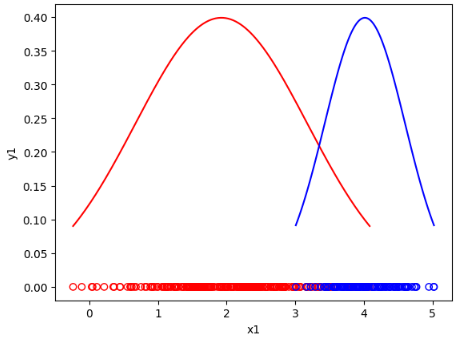
\includegraphics[width=0.5\linewidth]{generation_bayes.png}
    \caption{Geração de dados de acordo com as distribuições normais.}
    \label{fig:kernel_types}
 \end{figure}

 \newpage

 \section{Aplicação do algoritmo}

 O classificador bayesiano leva em consideração a independência entre os atributos, bem como a probabilidade a priori de ocorrência da classe ao realizar a classificação. Ele se baseia no teorema de Bayes, que é descrito pela seguinte equação:
 
 \[
P(C|X) = \frac{P(X|C) \cdot P(C)}{P(X)}
\]

O classificador, inicialmente, calcula a probabilidade de ocorrência de cada classe e, em seguida, multiplica esse resultado pela probabilidade da amostra pertencer a essa classe.

\section{Resultados}

Após aplicar o classificador bayesiano na base de dados simples, obtemos a seguinte matriz de confusão :

\begin{figure}[h]
    \centering
    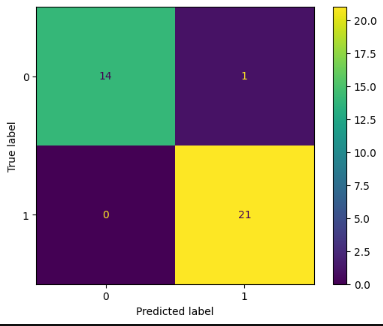
\includegraphics[width=0.5\linewidth]{conf_matrix_bayes.png}
    \caption{Matriz de confusão classificador de bayes.}
    \label{fig:kernel_types}
 \end{figure}

 O classificador obteve um bom desempenho pois as amostras seguem duas distribuições normais, com médias em 2 e em 4, e também pois as colunas são independentes entre si, levando o classificador a uma clara separação. A imagem abaixo mostra os dados separados em treino e em teste.

 \begin{figure}[h]
    \centering
    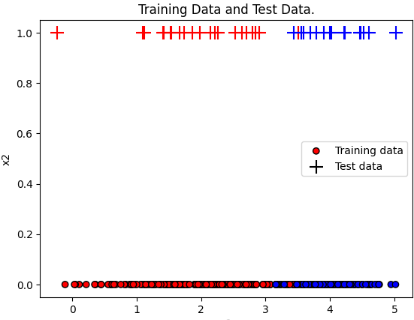
\includegraphics[width=0.5\linewidth]{train_test_points.png}
    \caption{Pontos divididos em treino e teste.}
    \label{fig:kernel_types}
 \end{figure}
 \newpage

\section{Conclusão}

Portanto, com esse relatório foi possivel introduzir conceitos relativos ao classificador bayesiano, cuja classificação se baseia no teorema de bayes e também na independência das colunas. É um classificador muito importante, pois é consideravelmente mais rápido do que os demais e também tem um bom desempenho para dados que seguem distribuições normais.
\end{document}
